\documentclass[border=10pt]{standalone}
\usepackage{pgfplots}
\pgfplotsset{compat=1.18}
\begin{document}
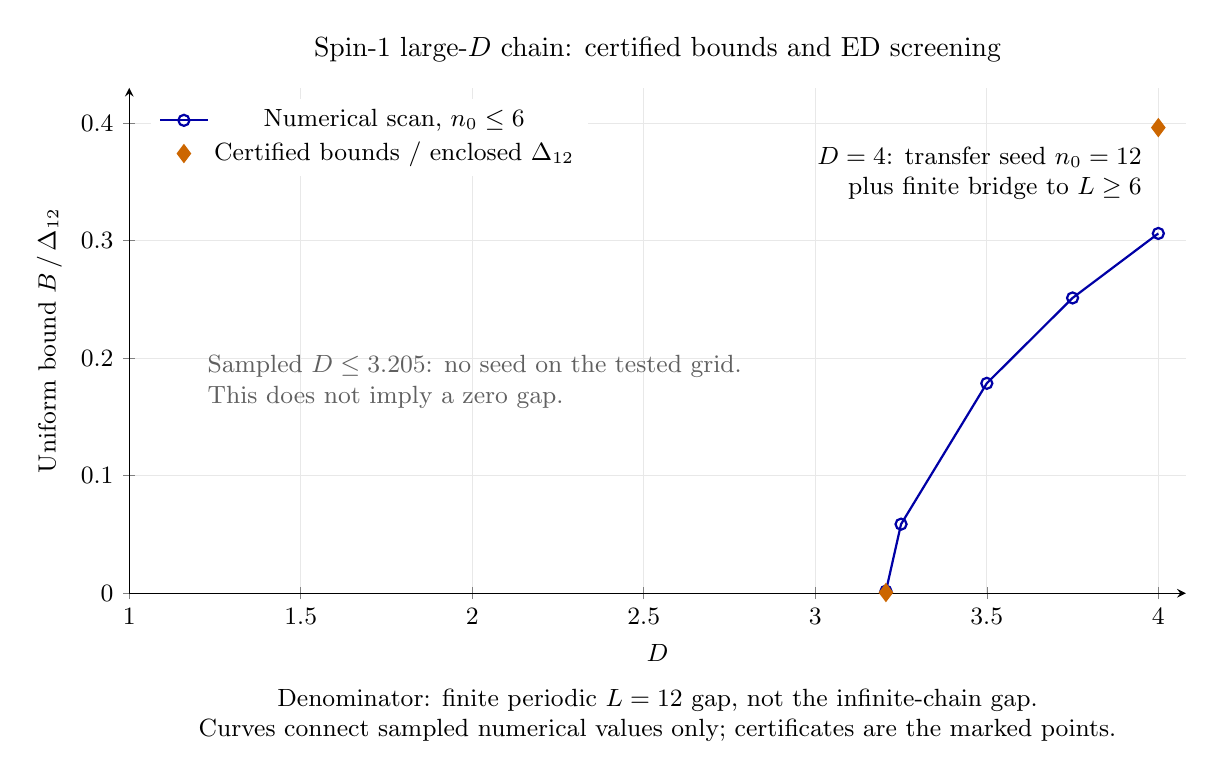
\begin{tikzpicture}
\begin{axis}[width=15cm,height=8cm,xmin=1,xmax=4.08,ymin=0,ymax=.43,
  xlabel={$D$},ylabel={Uniform bound $B\,/\,\Delta_{12}$},
  title={Spin-1 large-$D$ chain: certified bounds and ED screening},
  xtick={1,1.5,2,2.5,3,3.5,4},ytick={0,.1,.2,.3,.4},
  grid=major,grid style={gray!18},axis lines=left,clip=false,
  legend style={at={(.02,.98)},anchor=north west,draw=none,font=\small},
  tick label style={font=\small},label style={font=\small}]
\addplot[blue!65!black,thick,mark=o,mark options={fill=white}] coordinates {
(3.206,0.0018287170358027532)
(3.25,0.058782595333276684)
(3.5,0.17863631130628266)
(3.75,0.251250726042464)
(4.0,0.30613235710789277)};
\addlegendentry{Numerical scan, $n_0\le6$}
\addplot[orange!80!black,only marks,mark=diamond*,mark size=3.2pt] coordinates {
(3.2059998,0.0006481601371580482)
(4.0,0.3961914268603475)};
\addlegendentry{Certified bounds / enclosed $\Delta_{12}$}
\node[anchor=west,font=\small,align=left,text=gray!75!black]
  at (axis cs:1.2,.18)
  {Sampled $D\le3.205$: no seed on the tested grid.\\This does not imply a zero gap.};
\node[anchor=north east,font=\small,align=right] at (axis cs:3.98,.388)
  {$D=4$: transfer seed $n_0=12$\\plus finite bridge to $L\ge6$};
\node[anchor=north,font=\small,align=center] at (rel axis cs:.5,-.17)
  {Denominator: finite periodic $L=12$ gap, not the infinite-chain gap.\\
   Curves connect sampled numerical values only; certificates are the marked points.};
\end{axis}
\end{tikzpicture}
\end{document}
